In the framework of hand prosthetics, it is nowadays possible to build
mechanical hands possessing a fair amount of the abilities required by
the disabled to carry on living in a decent way. Modern hand
mechatronics has given us robotic hands which are highly humanoid,
light and gifted with a number of degrees of freedom. Attempts in this
sense include, e.g., the DLR prosthetic hand (\cite{Hua2006} --- see
Figure \ref{fig:DLRHandII}), the CyberHand project \cite{cyberhand},
and the i-LIMB hand by Touch Bionics \cite{ilimb}.

\begin{figure}
  \begin{tabular}{cc}
    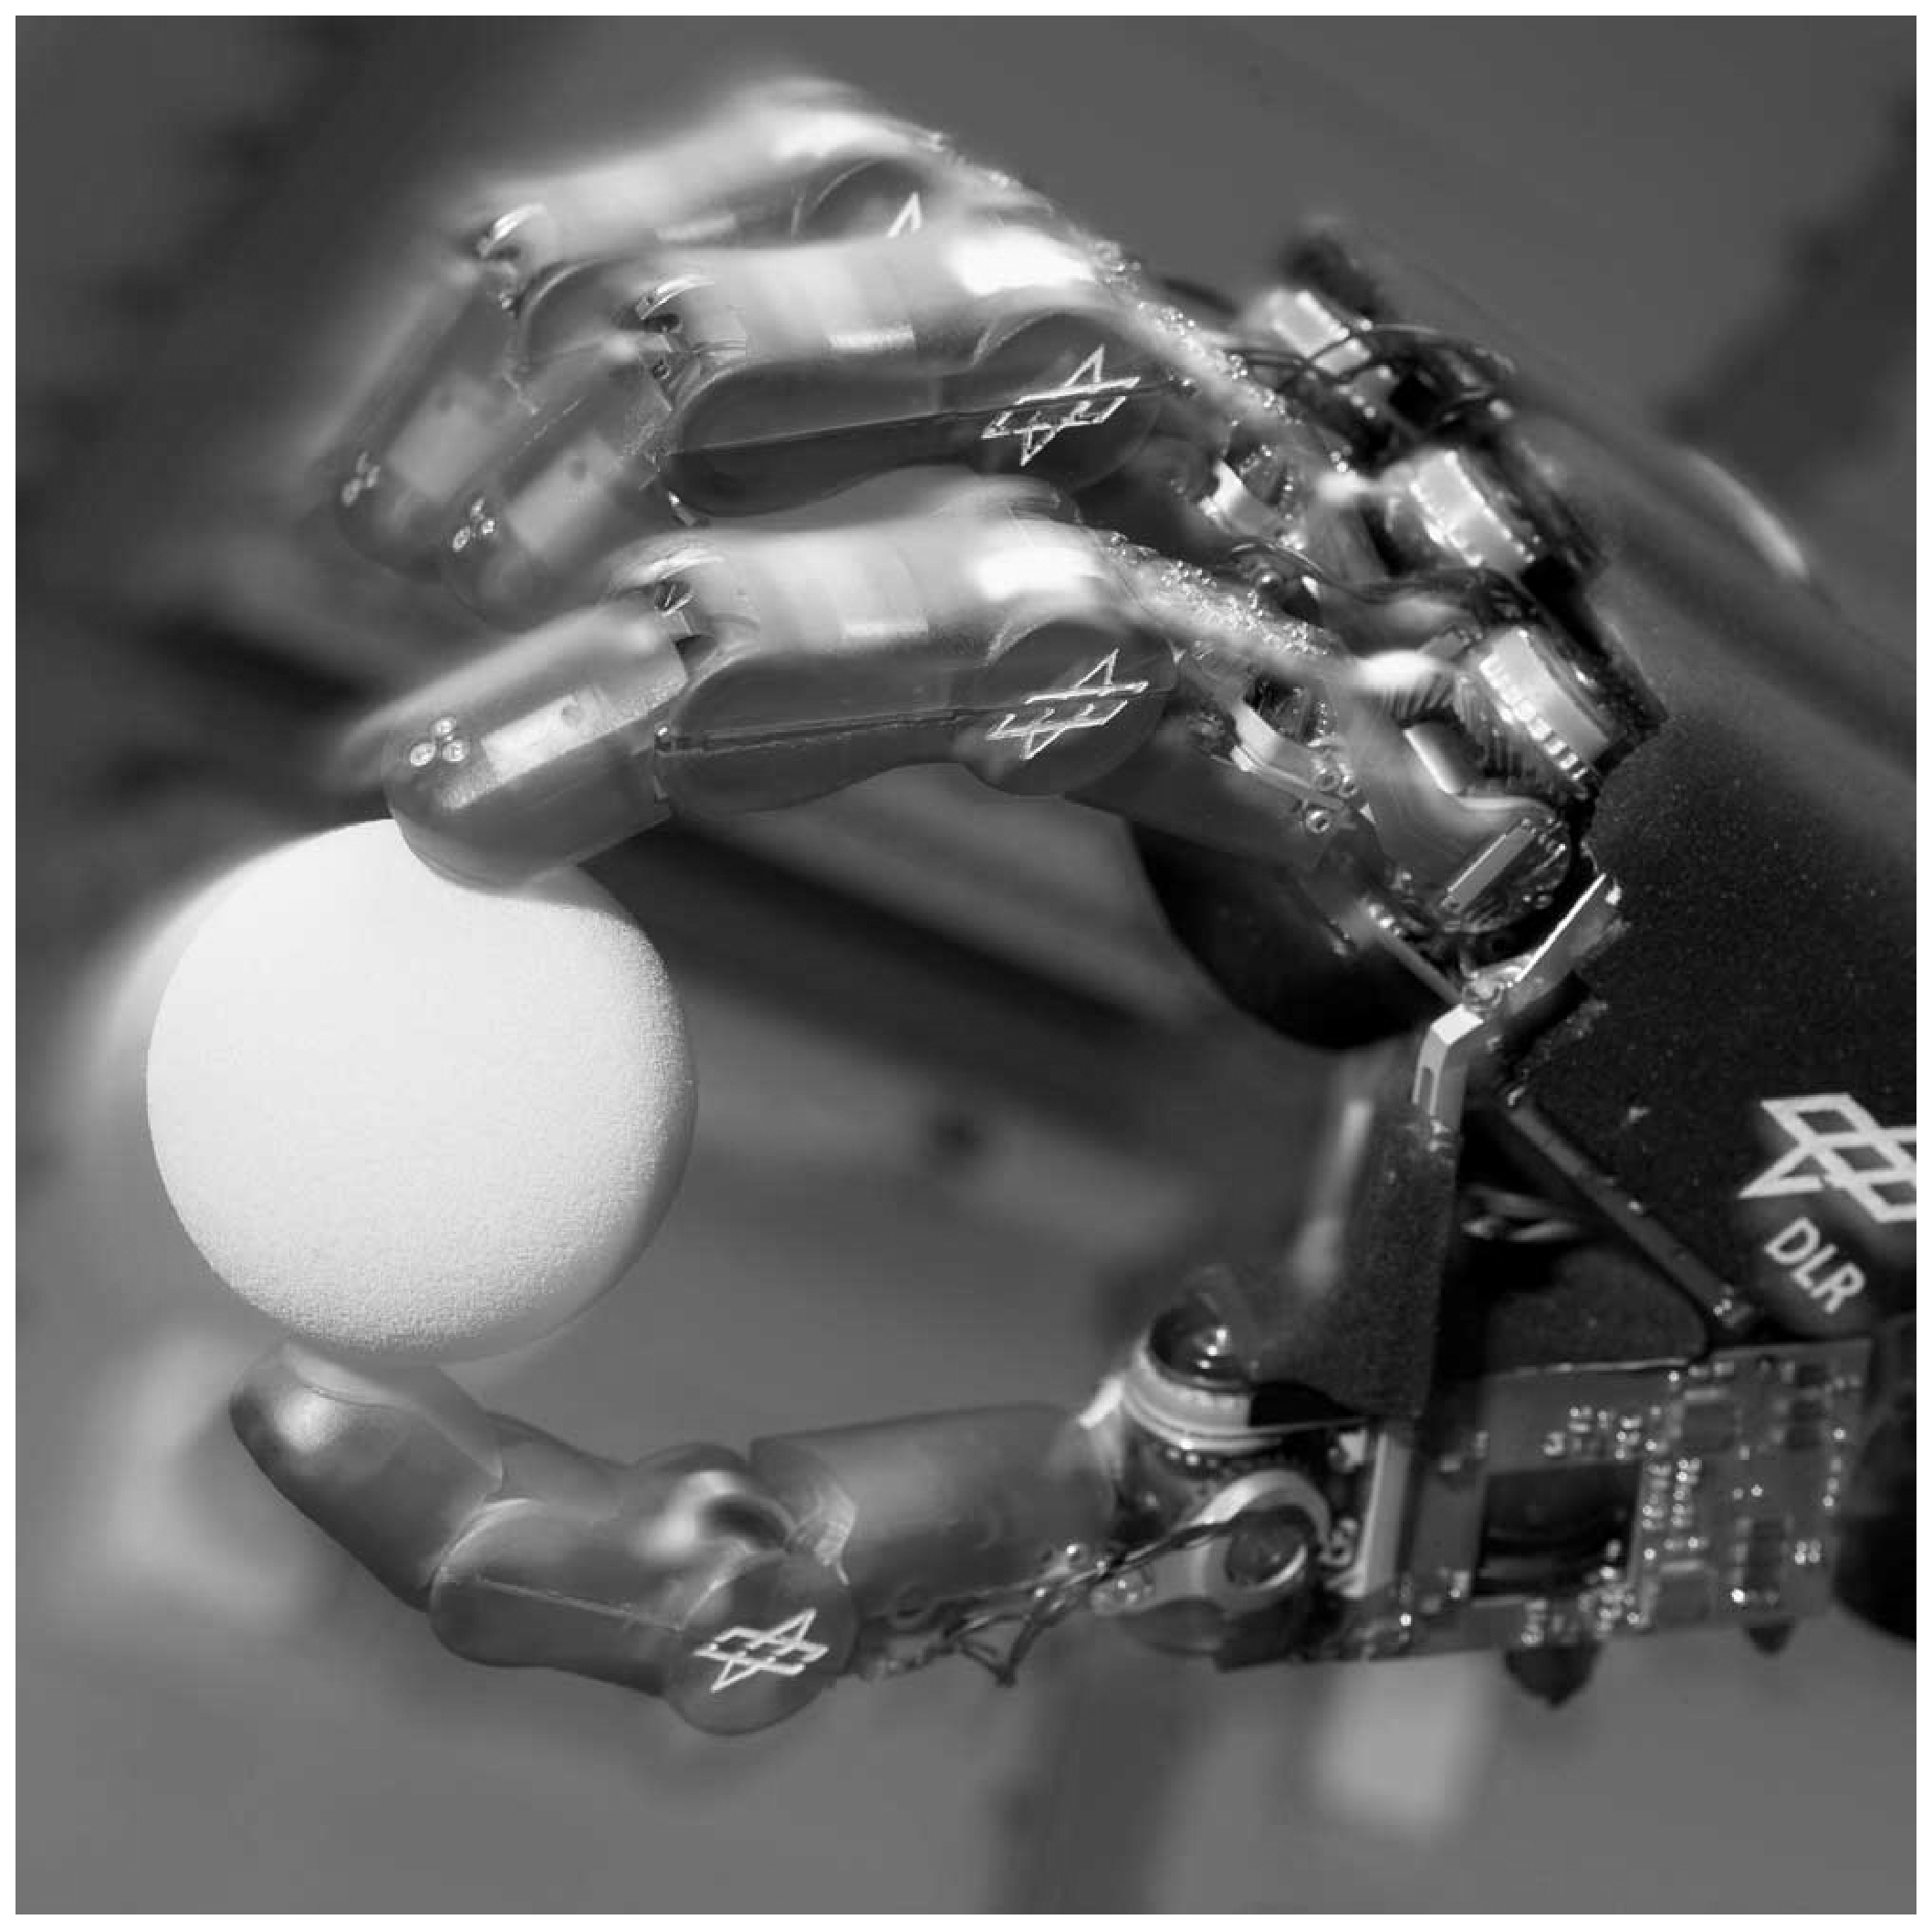
\includegraphics[height=0.12\textheight]{figs/DLRHand-Ball-comp.eps} &
    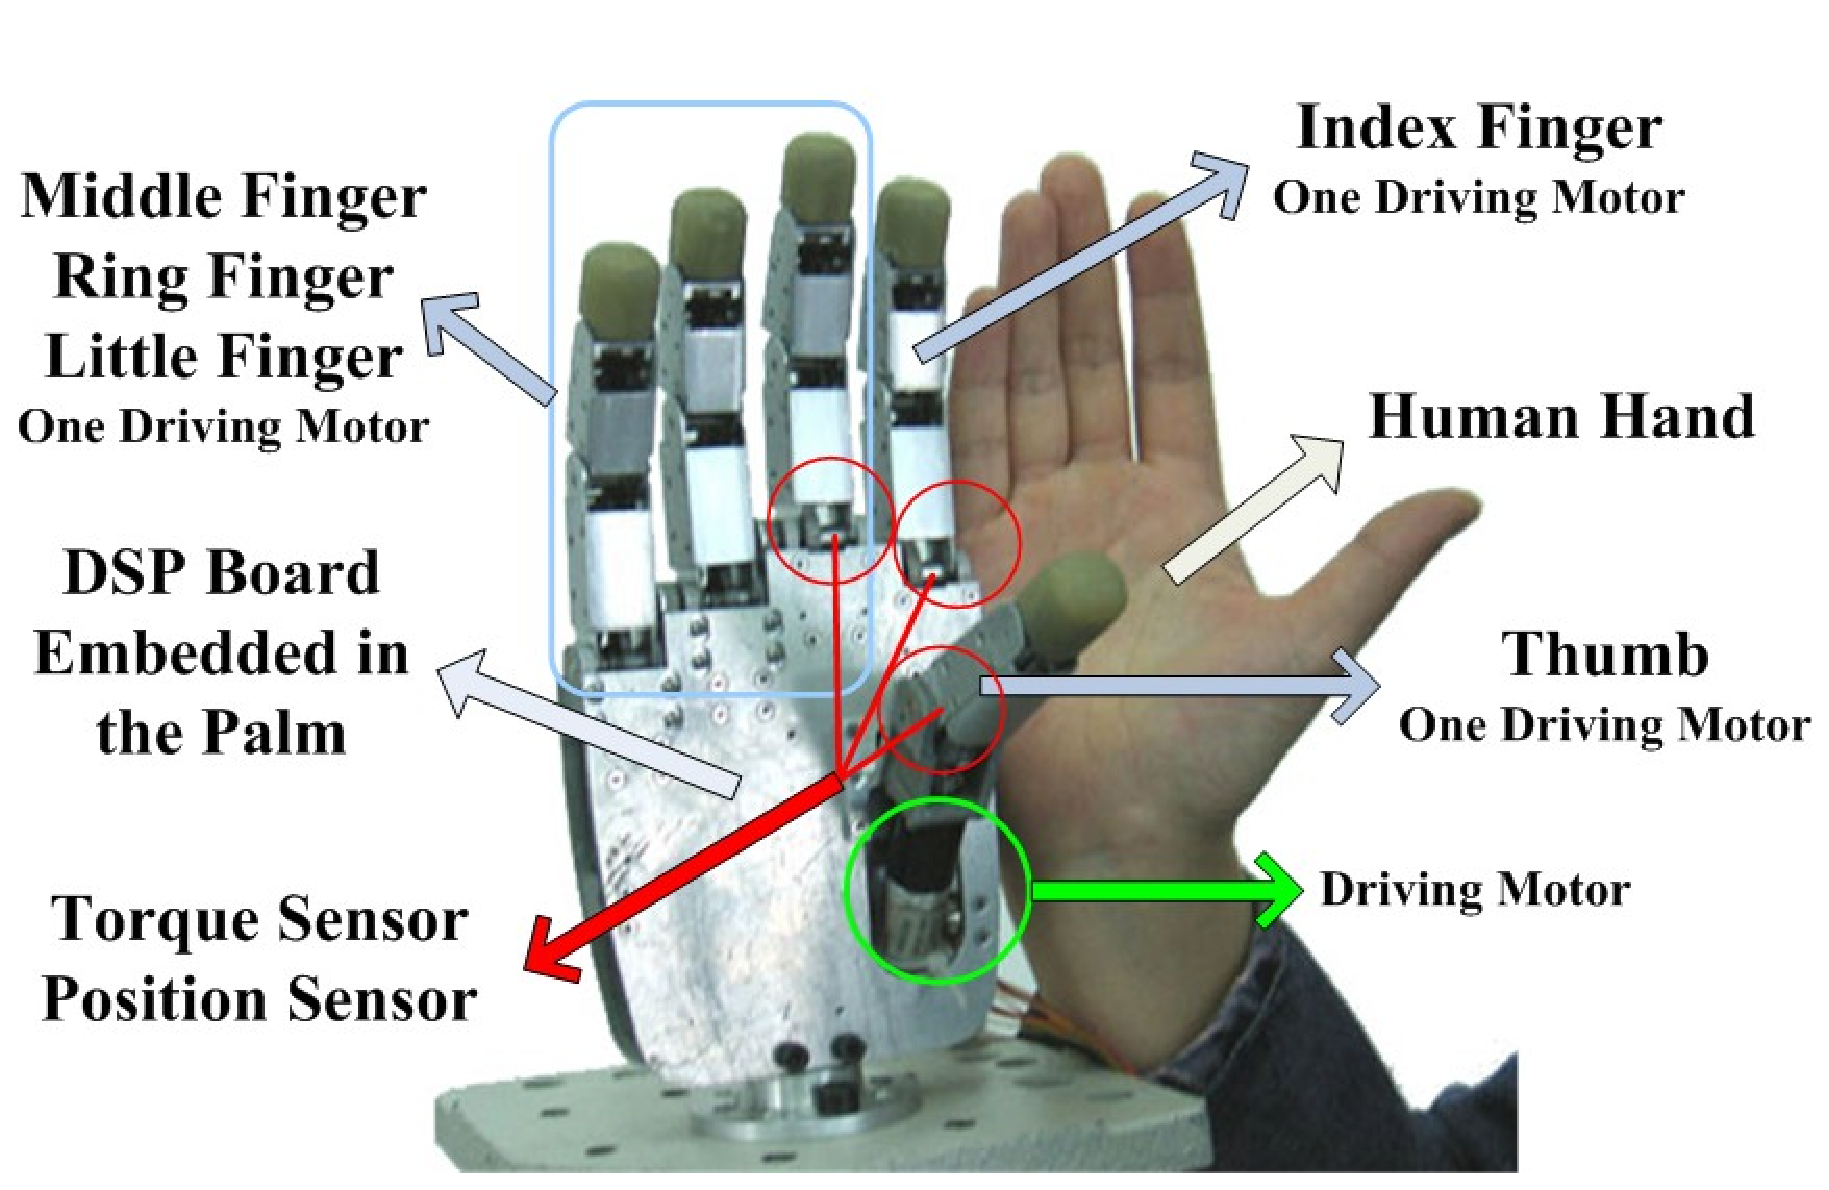
\includegraphics[height=0.12\textheight]{figs/DLR-Prothese.eps}
  \end{tabular}
  \caption{(left) The DLR Hand II. (right) The DLR prosthetic hand.}
  \label{fig:DLRHandII}
\end{figure}

Still, a general sense of frustration impends, as far as
\emph{control} of the prosthesis is concerned. As a matter of fact,
given the current state of the art, it is basically impossible for the
patient to precisely command the prosthesis what to do; whereas,
operating a hand requires a fine control down to the level of the
single fingers. First of all, presented with a certain task such as
turning a door handle or grabbing a car key, the patient must be able
to enforce the correct grasping type; this involves the activation of
some joints only, and in particular positions. Secondly, the amount of
force involved in the grasp must be controlled, so that it is possible
to grab, e.g., both a hammer without letting it slip and an egg
without breaking it.

To this end, two types of interfaces between the patient and the
prosthesis have been developed or are being studied: \emph{invasive}
and \emph{non-invasive}. The former gather control signals directly
from the user's nervous system, either via brain implants or surgical
use of electrodes. Quite obviously, invasive interfaces are supposed
to guarantee a high signal quality, since the signals can be gathered
exactly in the right spots; but they involve surgery and all related
sterility issues. On the other hand, non-invasive interfaces are
easier to handle, manufacture and implant, but require a much better
signal conditioning, since they usually work with surface (skin)
signals or vision and gaze tracking.

In the context of non-invasive interfaces for controlling mechanical
hands, a concrete possibility arises from \emph{forearm surface
electromyography (EMG)} \cite{zecca}, a technique by which muscle
activation potentials are gathered by electrodes placed on the
patient's forearm skin; these potentials can be used to track which
muscles the patient is willing to activate, and with what force.
Surface EMG is therefore, in principle, a cheap and easy way of
detecting what the patient wants the prosthesis to do.

Still, the EMG signal suffers from a number of problems, among which
the unprecise placement of the electrodes, signal drifting and change
due to sweat formation and muscular fatigue and cross-talking among
deep and superficial muscles. It seems, though, that good results can
be obtained via \emph{machine learning} techniques, as shown in, e.g.,
\cite{smagt}. In machine learning, one tries to approximate an unknown
function given its values in a number of samples; the application to
the current problem is exactly that of building a map relating EMG
activation potentials and muscle force, and therefore hand finger
movements. Such a system must be highly adaptive, accurate and fast
--- possibly, able to run in real time, as the patient is wearing the
prosthesis.

More in detail: so far, in literature, machine learning applied to
surface EMG has been able to \emph{classify} different postures of the
hand. For example, the surface EMG signal can be used to detect
whether the patient is attempting a cylindric grasp or a two-finger
grip \cite{ekvall}; but no indication about the amount of force
involved in the grasping act is detected, so that it is impossible to
distinguish between, e.g., a power grasp and a precision grip. We show
here a detailed comparative analysis of what machine learning can do
when applied to such a problem. Over two days, we have gathered
forearm surface EMG data while the subject was gripping in four
distinct ways a force sensor; we have then trained three different
machine learning systems to guess, from the EMG signal,

\begin{enumerate}

  \item what kind of grasp the subject was doing, e.g., thumb and
    index finger, thumb and middle finger, thumb and ring finger or
    thumb and all other fingers; and

  \item how much force the subject was applying to the sensor, in
    order to understand whether the grasp was a power grasp or rather
    a precision grip.

\end{enumerate}

Surprisingly, as far as we know, nobody has ever attempted so far to
solve problem $2$. The three approaches we have experimented with are:
$(a)$ a simple feed-forward neural network with one hidden layer,
$(b)$ a Support Vector Machine with radial basis function kernel
\cite{BGV92}, $(c)$ Locally Weighted Projection Regression
\cite{lwpr}. Our analysis consists of a preliminary phase in which
several models have been built in a batch fashion, in order to
understand how to deal with the non-stationarity of EMG. The most
interesting challenge has been how to filter out unwanted data, at the
same time keeping a high overall accuracy, both in classification and
regression. Later on, based upon the results obtained in the
preliminary phase, we have developed a simple but effective procedure
for selecting a subset of the samples on-the-fly, called \emph{Online
Uniformisation} (OU).

OU is based upon the simple idea of keeping a minimum inter-sample
Euclidean distance, in order to uniformly sample the input space. The
selected samples are then used to periodically re-train the system,
and check that it has adapted to the new data. The training sets so
obtained are remarkably small and thus usable on-line, and they offer
an excellent trade-off between size and accuracy. In particular, while
the size of the uniform training sets decays polynomially, the error
rates seems to increase only linearly. This behaviour appears in both
problems highlighted above (the former involving classification, the
latter regression), and for all the approaches tested. Our numerical
results indicate that, in such a scenario, the type of grasp can be
reconstructed with an average accuracy of $89.67\% \pm 1.53\%$, and
the applied force can be predicted with an average percentage error of
$7.89\% \pm 0.09\%$, meaning $4.5$N over a range of about $57$N.

The paper is structured as follows: after a brief review of relevant
literature, we describe in detail the experiment and the methods used
to tackle it (Section \ref{sec:m&ms}); then we show and comment on the
experimental results, both the preliminary phase and the online
experiments (Section \ref{sec:exp}); lastly, discussion and
conclusions are presented.
